\documentclass[expanded]{lkx_pset}

\title{CS181 Problem Set 0}
\author{Lev Kruglyak}
\due{January 26, 2024}

\usepackage{pgfplots}
\pgfplotsset{compat=1.14}
\usepackage[outputdir=build]{minted}
\usepackage{graphicx}

\collaborator{AJ LaMotta}

\begin{document}
\maketitle

\begin{problem}{1}[Modeling Linear Trends - Linear Algebra Review]
Let's consider a dataset consisting of two points $\mathcal{D} = \{(x_1, y_1), (x_2, y_2)\}$, where $x_n, y_n$ are scalars for $n=1, 2$. Recall that the equation of a line in 2-dimensions can be written: $y = w_0 + w_1x$. 
\end{problem}

\begin{parts}
  \begin{part}{a}
    Write a system of linear equations determining the coefficients $w_0, w_1$ of the line passing through the points in our dataset $\mathcal{D}$ and analytically solve for $w_0, w_1$ by solving this system of linear equations (i.e., using substitution). Please show your work.
  \end{part}

  Suppose that the line $y= w_0 + w_1x$ passes through the points $(x_1, y_1)$ and $(x_2, y_2)$. By definition, this gives us the system of equations:
  \[
    \begin{cases}
      y_1 = w_0 + w_1 x_1,\\ y_2 = w_0 + w_1 x_2.
    \end{cases}
  \]
  Solving for the coefficients $w_1$ by substitution, we get
  \[
    w_0 = y_1 - w_1x_1, \quad w_0 = y_2 - w_1 x_2 \quad\implies\quad w_1 = \frac{y_2 - y_1}{x_2 - x_1}.
  \]
  Then plugging this back into the equation, we get
  \[
    y_1 = w_0 + \frac{y_2-y_1}{x_2 - x_1}\cdot x_1 \quad\implies\quad w_0 = y_1 - \frac{y_2 - y_1}{x_2 - x_1}\cdot x_1.
  \]
  In particular, a solution to this system requires that $x_1\neq x_2$, since otherwise the slope coefficient ($w_1$) would be infinite and there would not be an analytic solution.

  \begin{part}{b}
    Write the above system of linear equations in matrix notation, so that you have a matrix equation of the form $\mathbf{y} = \mathbf{X}\mathbf{w}$, where $\mathbf{y}, \mathbf{w} \in \mathbb{R}^2$ and $\mathbf{X} \in \mathbb{R}^{2\times 2}$. 
    For full credit, it suffices to write out what $\mathbf{X}$, $\mathbf{y}$, and $\mathbf{w}$ should look like in terms of $x_1$, $x_2$, $y_1$, $y_2$, $w_0$, $w_1$, and any other necessary constants. Please show your reasoning and supporting intermediate steps.
  \end{part}

  Alternatively, we could write out this system of equations as
  \[
    \begin{cases}
      y_1 = w_0 + w_1 x_1,\\ y_2 = w_0 + w_1 x_2
    \end{cases}\quad \implies\quad \begin{bmatrix}y_1\\y_2\end{bmatrix} = \begin{bmatrix} w_0 + w_1x_1\\ w_0 + w_1 x_2\end{bmatrix} = \begin{bmatrix}1&x_1\\1&x_2\end{bmatrix}\begin{bmatrix}w_0\\w_1\end{bmatrix}.
  \]
  Thus, we can set
  \[
    \mathbf{y}=\begin{bmatrix}y_1\\y_2\end{bmatrix},\quad \mathbf{X}=\begin{bmatrix}1&x_1\\1&x_2\end{bmatrix}, \quad \mathbf{w}=\begin{bmatrix}w_0\\w_1\end{bmatrix}
  \]
  so that our system becomes $\mathbf{y}=\mathbf{X}\mathbf{w}$.

  \begin{part}{c}
    Using properties of matrices, characterize exactly when an unique solution for  $\mathbf{w}=\left(w_0 \; w_1 \right)^{T}$ exists. In other words, what must be true about your dataset in order for there to be a unique solution for $\mathbf{w}$? When the solution for $\mathbf{w}$ exists (and is unique), write out, as a matrix expression, its analytical form (i.e., write $\mathbf{w}$ in terms of $\mathbf{X}$ and $\mathbf{y}$).
%     Hint: What special property must our $\mathbf{X}$ matrix possess? What must be true about our data points in $\mathcal{D}$ for this special property to hold?
  \end{part}

  For there to be a unique solution to the system, the matrix $\mathbf{X}$ must be invertible, since then $\mathbf{w} = \mathbf{X}^{-1}\mathbf{y}$. This is equivalent to $\mathbf{X}$ having non-zero determinant, which in our case means
  \[
    \begin{vmatrix}1&x_1\\1&x_2\end{vmatrix}=x_2 - x_1\neq 0 \quad\implies\quad x_1\neq x_2.
  \]
  This is the exact condition we got before.

  \begin{part}{d}
    Compute $\mathbf{w}$ by hand via your matrix expression in (c) and compare it with your solution in (a). Do your final answers match? What is one advantage for phrasing the problem of fitting the model in terms of matrix notation? 
  \end{part}

  First, let's compute the inverse $\mathbf{X}^{-1}$. This has analytic form
  \[
    \mathbf{X}^{-1} = \frac{1}{x_2 - x_1}\begin{bmatrix}x_2 & -x_1\\ -1 & 1\end{bmatrix}.
  \]
  Then, solving for $\mathbf{w}$ we get
  \[
    \mathbf{w} = \mathbf{X}^{-1}\mathbf{y} = \frac{1}{x_2 - x_1}\begin{bmatrix}x_2 & -x_1\\ 1 & 1\end{bmatrix}\begin{bmatrix}y_1\\ y_2\end{bmatrix} = \begin{bmatrix} (x_2 y_1 - y_2 x_1)/(x_2-x_1)\\ (y_2 - y_1)/(x_2 - x_1)\end{bmatrix}.
  \]
  These are the same expressions we derived in the previous problem parts, albeit in a simplified form. One advantage to using matrix notation is easier generality for higher dimensions, i.e. when there are more points in the dataset.

  \begin{part}{e}
    In real-life, we often work with datasets that consist of hundreds, if not millions, of points. In such cases, does our analytical expression for $\mathbf{w}$ that we derived in (3) apply immediately to the case when $\mathcal{D}$ consists of more than two points? Why or why not?
  \end{part}

  No, the analytic expression does not immediately generalize. Firstly, given some set of more than $2$ data points, there might not even be a line which passes through all of them, so we would need a different model.
\end{parts}

\begin{problem}{2}[Optimizing Objectives - Calculus Review]
   In her most recent work-from-home shopping spree, Nari decided to buy several house plants. \textit{Her goal is to make them to grow as tall as possible.} After perusing the internet, Nari learns that the height $y$ in mm of her Weeping Fig plant can be directly modeled as a function of the oz of water $x$ she gives it each week:
$$y = - 3x^2 + 72x + 70.$$
\end{problem}

\begin{parts}
  \begin{part}{a}
    Based on the above formula, is Nari's goal achievable: does the plant have a maximum height? Why or why not? Does her goal have a unique solution - i.e. is there one special watering schedule that would acheive the maximum height (if it exists)?

    % Hint: plot this function. In your solution, words like ``convex" and ``concave" may be helpful.
  \end{part}

  This function has the form of an inverted parabola, so it has a global maximum, and this is clear from the graph:

  \begin{figure}[ht]
    \centering
    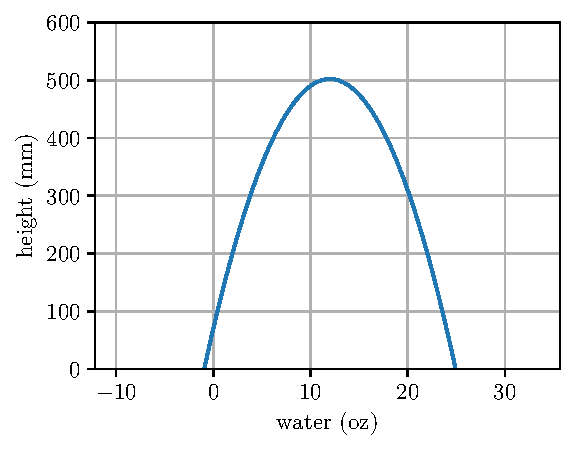
\includegraphics[]{build/2a.pdf}
  \end{figure}\noindent
  Furthermore, there is only one local maximum since the equation $y'=-6x+72=0$ has only one solution.

  \begin{part}{b}
    Using calculus, find how many oz per week should Nari water her plant in order to maximize its height. With this much water, how tall will her plant grow?

    % Hint: solve analytically for the critical points of the height function (i.e., where the derivative of the function is zero).  For each critical point, use the second-derivative test to identify if each point is a  max or min point, and use arguments about the global structure (e.g., concavity or convexity) of the function to argue whether this is a local or global optimum.
  \end{part}

  The unique critical point of this function is the solution to $y'=0$, which here means
  \[
    -6x+72 = 0 \quad\implies \quad x = 12.
  \]
  Since the second derivative is $y''=-6$, by the second derivative test this is a concave function and 
  thus the optimal water quantity is 12 oz. Plugging this back in, we see that the plant will grow to a height of 502 mm.

  \begin{part}{c}
    Now suppose that Nari want to optimize both the amount of water $x_1$ (in oz) \textit{and} the amount of direct sunlight $x_2$ (in hours) to provide for her plants. After extensive research, she decided that the height $y$ (in mm) of her plants can be modeled as a two variable function:

    $$y = f(x_1, x_2) = \exp\left(-(x_1 - 2)^2 - (x_2 - 1)^2 \right)$$
    Using \texttt{matplotlib}, visualize in 3D the height function as a function of $x_1$ and $x_2$ using the \texttt{plot\_surface} utility for $(x_1, x_2) \in (0, 6) \times (0, 6)$. 
    Use this visualization to argue why there exists a unique solution to Nari's optimization problem on the specified intervals for $x_1$ and $x_2$.
  \end{part}

  Using \texttt{matplotlib}, we can generate the following 3d plot of the function:

  \begin{figure}[ht]
    \centering
    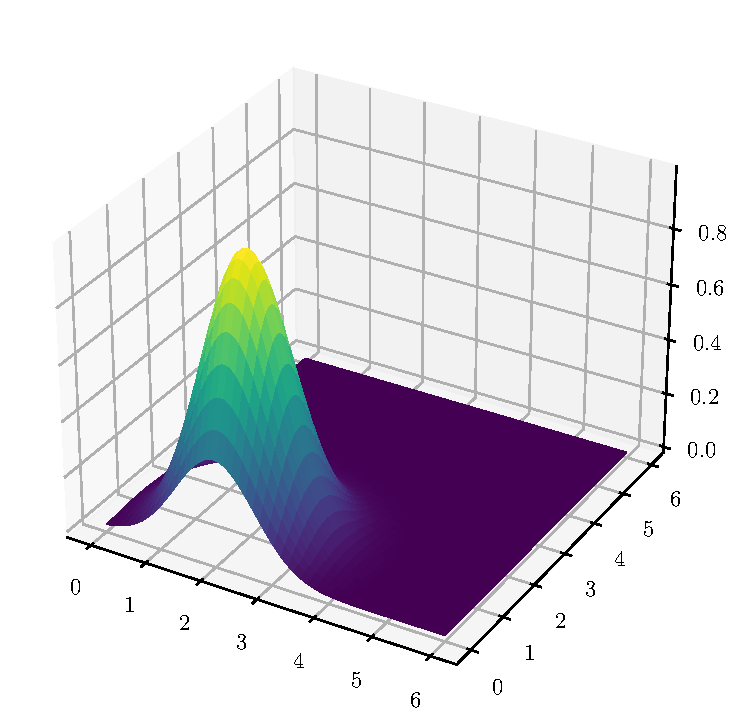
\includegraphics[]{build/2b.pdf}
  \end{figure}\noindent

  This clearly has a single peak where the maximum occurs. Reasoning analytically, we note that $f$ consists of a inverted parabaloid $-(x_1-2)^2 - (x_2 - 1)^2$ (which has a maximum at $(2,1)$) composed with a strictly-increasing function $\exp$. This means that $f$ also has a unique maximum at $(2, 1)$.
\end{parts}


\begin{problem}{3}[Reasoning about Randomness - Probability and Statistics Review]
Consider the following model for packages arriving at the US Postal Service (USPS):
\begin{itemize}
    \item Packages arrive randomly in any given hour according to a Poisson distribution. That is, the number of packages in a given hour $N$ is distributed $\textrm{Pois}(\lambda)$, with $\lambda = 3$.
    \item Each package has a random size $S$ (measured in $in^3$) and weight $W$ (measured in pounds), with joint distribution
    $$(S, W)^{T} \sim \mathcal{N}\left( \boldsymbol{\mu}, \boldsymbol{\Sigma}\right) \text{, with } \boldsymbol{\mu} = \begin{bmatrix} 120 \\ 4 \end{bmatrix} \text{ and } \boldsymbol{\Sigma} = \begin{bmatrix} 1.5 & 1 \\ 1 & 1.5 \end{bmatrix}.$$
    \item Processing time $T$ (in seconds) for each package is given by $T = 60 + 0.6 W + 0.2 S + \epsilon$, where $\epsilon$ is a random noise variable with Gaussian distribution $\epsilon \sim \mathcal{N}(0, 5)$.
\end{itemize}
For this problem, you may find the \texttt{multivariate\_normal} module from \texttt{scipy.stats} especially helpful. You may also find the \texttt{seaborn.histplot} function quite helpful. 
\end{problem}

\begin{parts}
  \begin{part}{a}
    Perform the following tasks.

    \begin{enumerate}
        \item Visualize the Bivariate Gaussian distribution for the size $S$ and weight $W$ of the packages by sampling 500 times from the joint distribution of $S$ and $W$ and generating a bivariate histogram of your $S$ and $W$ samples.
        \item Empirically estimate the most likely combination of size and weight of a package by finding the bin of your bivariate histogram (i.e., specify both a value of $S$ and a value of $W$) with the highest frequency. A visual inspection is sufficient -- you do not need to be incredibly precise.  How close are these empirical values to the theoretical expected size and expected weight of a package, according to the given Bivariate Gaussian distribution?
    \end{enumerate}
  \end{part}

  Using \texttt{matplotlib} and the \texttt{multivariate\_normal} module, we obtain the following bivariate histogram:

  \begin{figure}[ht]
    \centering
    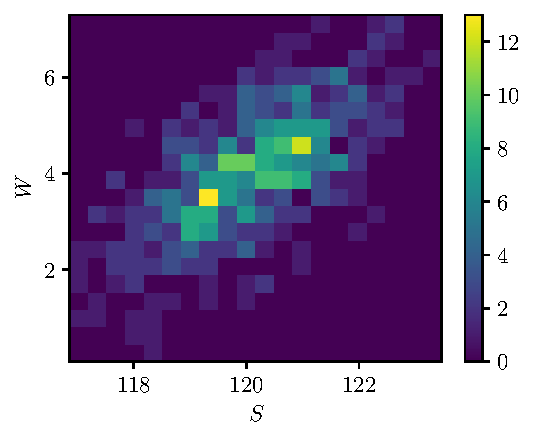
\includegraphics[]{build/3a.pdf}
  \end{figure}\noindent
  From this figure, it looks like the most likely combination of size and weight is thus $(S,W)=(119.5, 3.8)$ which is fairly close to the mean of $(120, 4)$.

  \begin{part}{b}
     For 1001 evenly-spaced values of $W$ between $0$ and $10$, plot $W$ versus the joint Bivariate Gaussian PDF $p(W, S)$ with $S$ fixed at $S=118$. Repeat this procedure for $S$ fixed at $S=122$. Comparing these two PDF plots, what can you say about the correlation of random variables $S$ and $W$?
  \end{part}

  Using the same \texttt{multivariate\_normal} module, we obtain the following PDFs:

  \begin{figure}[ht]
    \centering
    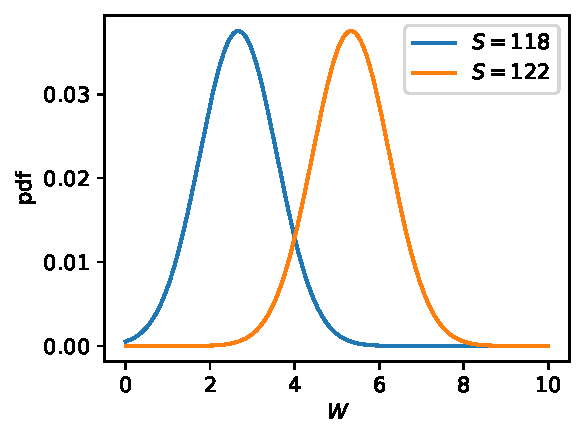
\includegraphics[]{build/3b.pdf}
  \end{figure}\noindent
  Since these PDFs of $W$ are distinct when we condition on $S$, this means that $S$ and $W$ are correlated.

  \begin{part}{c}
     Give one reason for why the Gaussian distribution is an appropriate model for the size and weight of packages. Give one reason for why it may not be appropriate.
  \end{part}

  By the central limit theorem, sums of (nice enough) random variables coverge to a Gaussian distribution, thus making it common in many real world scenarios. Furthermore, we can a slight correlation between weight and size since there isn't too much of a variation in package density.

  One way in which it might be not as appropriate is if there is a ``skew'' in the distribution of package weights, for example there might be many more light packages, with a tapering distribution of heavier packages, but a much sharper dropoff for ``weightless'' packages.

  \begin{part}{d}
    Because $T$ is a linear combination of random variables, it itself is a random variable. Using properties of expectations and variance, please compute $\mathbb{E}(T)$ and $\mathrm{Var}(T)$ analytically.
  \end{part}

  Due to linearity of expectation, we can expand the expectation as
  \[
    \begin{aligned}
      \mathbb{E}(T) &= \mathbb{E}(60)+0.6\mathbb{E}(W) + 0.2\mathbb{E}(S)+\mathbb{E}(\epsilon) = 60+0.6\cdot 4 + 0.2\cdot 120 + 0 = 86.4.
    \end{aligned}
  \]
  Similarly, we can expand the variance as 
  \[
    \begin{aligned}
      \mathrm{Var}(T) &= \mathrm{Var}(60)+0.6^2\cdot \mathrm{Var}(W) + 0.2^2\cdot \mathrm{Var}(S)+\mathrm{Var}(\epsilon) = 0 + 0.6^2\cdot 1.5 + 0.2^2\cdot 1.5 + 5 = 5.84.
    \end{aligned}
  \]

  \begin{part}{e}
     Let us treat the \textit{total} amount of time it takes to process \textit{all} packages received at the USPS office within \textit{an entire day} (assuming a single day is $24$ hours long) as a random variable $T^{*}$. 
    \begin{enumerate}
        \item Write a function to simulate draws from the distribution of $T^{*}$. 
        \item Using your function, empirically estimate the mean and standard deviation of $T^{*}$ by generating $1000$ samples from the distribution of $T^{*}$.
    \end{enumerate}
  \end{part}

  We produce the following commented functions in Python to sample $T$ and $T^*$:
  \begin{minted}[fontfamily=tt]{python}
    import numpy as np

    def sample_T(packages):
        sw_samples = np.random.multivariate_normal([120, 4], [[1.5, 1], [1,1.5]], packages)
        e_samples = np.random.normal(0, np.sqrt(5), packages)
        return np.sum(60 + 0.6 * sw_samples[:, 1] + 0.2 * sw_samples[:, 0] + e_samples)


    def sample_T_star(num_samples):
        times = []

        for _ in range(num_samples):
            # List of number of packages arriving every hour
            packages_samples = np.random.poisson(3, 24)
            total = 0

            # Simulate size, weight, and processing time for each package
            for packages in packages_samples:
                total += sample_T(packages)

            times.append(total)

        return np.mean(times), np.std(times)
  \end{minted}

  By generating 1000 samples, we can use \texttt{numpy} to take the mean and standard deviation of the samples, thus getting estimates for the mean and standard deviation of $T$ and $T^*$. These estimates are:
  \[\mathbb{E}(T^*) = 6226.25, \quad \sigma_{T^*} = 710.60. \]
\end{parts}

\end{document}
